\chapter{Protocol Design}
\label{chap:protocoldesign}

In the state of the art, there are different protocols constructed over \ac{IEEE} 802.15.4, like ZigBee, WirelessHART, 6LoWPAN \ldots \ some
are prepared for low consumption, others build different applications, but almost none of them are focused in localization. In the
department \ac{LPL} and \ac{OLP} \cite{LPLandOLP} protocols were proposed for this purpose. This protocols are based in \ac{IEEE} 802.15.4 and specifically 
designed for localization. In the next section a brief overview will be given, for a deeper view, please consult \cite{LPLandOLP}.

\section{\ac{LPL} and \ac{OLP}}

\ac{LPL} and \ac{OLP} \cite{LPLandOLP}, are two protocols designed for localization and based in \ac{RSSI} values. This values give an idea of 
the received signal strength in the device, and have the advantage that this information is already in all packets a device receives, there
is no need of special hardware or data to be prepared or obtained like in other methods (ultra wide band for example). But \ac{RSSI} values have 
a big problem for localization, its dispersion is very big, making the localization resolution (in some cases up to many meters 
\cite{fingerprint}) bad for some applications. 

This resolution problem, can be solved through some approaches. One kind is using localization techniques like ``fingerprint 
technique'' \cite{fingerprint} that improves the resolution. Another option is, taking more than 1 \ac{RSSI} value to obtain a more stable 
result. This technique has one big challenge, the more values are taken, the higher the energy consumption. Without a good approach, 
the \ac{MN} would need to listen to the channel most of the time waiting to receive packets from \ac{AN} to obtain \ac{RSSI} values, 
this way a lot of energy would be wasted just doing nothing, this is called idle listening. This 2 protocols propose 2 different 
approaches to solve this.

Another aspect in localization is who calculates the position, 3 different alternatives can be obtained.

\begin{itemize}
 \item \textbf{Centralized.} A central computer receives the \ac{RSSI} values from all \acp{AN} in the network and calculates the positions of 
the \acp{MN}. The advantage is that the computer can use complicate algorithms to obtain better results, but this method 
charges the network with a lot of traffic, specially if the \ac{MN} needs to know its position back after calculation.
 \item \textbf{Distributed-A.} The \ac{MN} sends the \ac{RSSI} values directly to the \ac{AN}, and this calculates directly the \ac{MN} position,
this does not charge the network so much like the centralized approach but the resolution is also not so good. It is important to note that 
each \ac{MN} has a ``selected \ac{AN}'', this \ac{AN} is the one in charge to calculate \ac{MN} position and the one the \ac{MN} communicates
with and through. This \ac{AN} is usually the one closest to the \ac{MN}.
 \item \textbf{Distributed-M.} In this mode, is the \ac{MN} who calculates directly its position from \ac{RSSI} values obtained from \acp{AN},
the problem is that \acp{MN} cannot use powerful localization algorithms. This solution is the one that almost does not charge the network.
\end{itemize}

The protocols \ac{LPL} and \ac{OLP} are going to use phases for different behaviors, and this phases will be repeated cyclically, that's why 
a good synchronization among all the nodes is necessary so all nodes can start the phases at the same time. Nodes will get 
the synchronization information from their parents (do not forget that a tree topology is used) using an active or a passive synchronization. 
To get a graphical explanation check Figure \ref{fig:synchronization}.

\begin{itemize}
 \item \textbf{Passive Synchronization.} The parent starts the process sending a packet R1 to \ac{MAC} to be transmitted, this packet is
created at the time-stamp Tx1, and includes this time, the time until the next phase start (TF) and info about this phase. Due to random time in 
\ac{CSMA/CA} process and other processing times, R1 is not transmitted immediately but in Tx2. When the packet is transmitted, \ac{MAC} informs
the application layer and this creates another packet (R2) including the new time-stamp Tx2. At the child, 2 packets will be received, R1 and 
R2 in times Rx1 and Rx2 respectively. Calculation of next phase start from the child point of view (TZ) is done like in (\ref{mat:pasivesync}).

\begin{equation}
  TZ = TF - (Rx2 - Rx1) - (Tx2 - Tx1)
  \label{mat:pasivesync}
\end{equation}

\begin{figure}[here]
 \begin{center}
  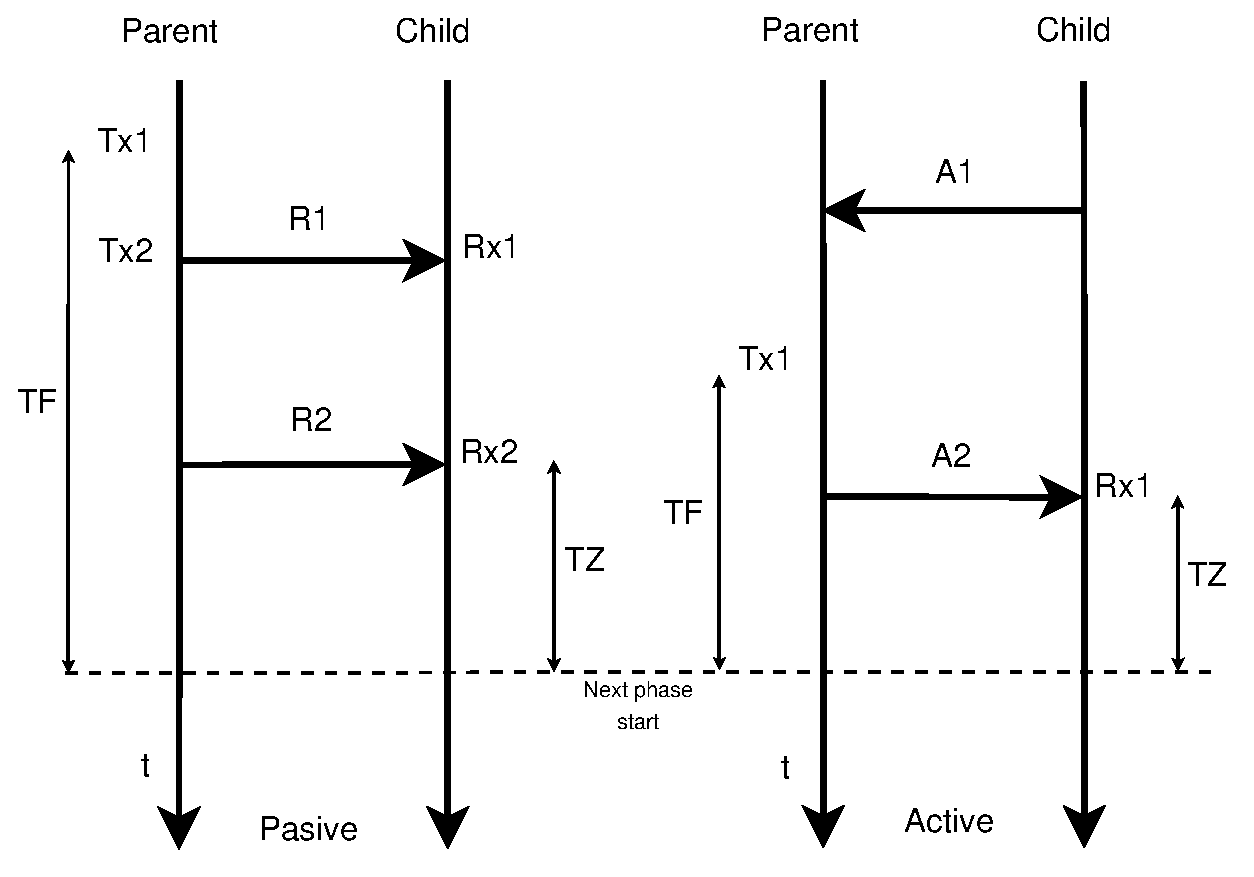
\includegraphics[width=0.6\textwidth]{synchronization.eps}
 \end{center}
 \caption{Passive and Active Synchronization \cite{LPLandOLP}}
 \label{fig:synchronization}
\end{figure}
 
 \item \textbf{Active Synchronization.} In the active synchronization, the child starts the process sending a synchronization request (A1),
then the parent answers with packet A2, this packet contains the time until the start of the next phase (TF). The child can calculate this time
with like in (\ref{mat:activesync}).

\begin{equation}
  TZ = TF - C
 \label{mat:activesync}
\end{equation}

The C parameter in (\ref{mat:activesync}), represents an estimation of all the processing times and random times from \ac{CSMA/CA}, that is why
this method is not so exact like the passive one, although it does not need 2 packets like it.
\end{itemize}

In the following subsections, both protocols \ac{LPL} and \ac {OLP} are going to be introduced.

\subsection{\acl{LPL}}

To reduce the idle listening, and thus the energy consumption, this protocol, proposes that instead of listening to the \acp{AN}, the
\acp{MN} are the ones who transmit and the \acp{AN} the ones who listen and transmit this information. This protocol is divided in 3 
phases which can be appreciated in Figure \ref{fig:LPL}.

\begin{figure}[h]
 \begin{center}
  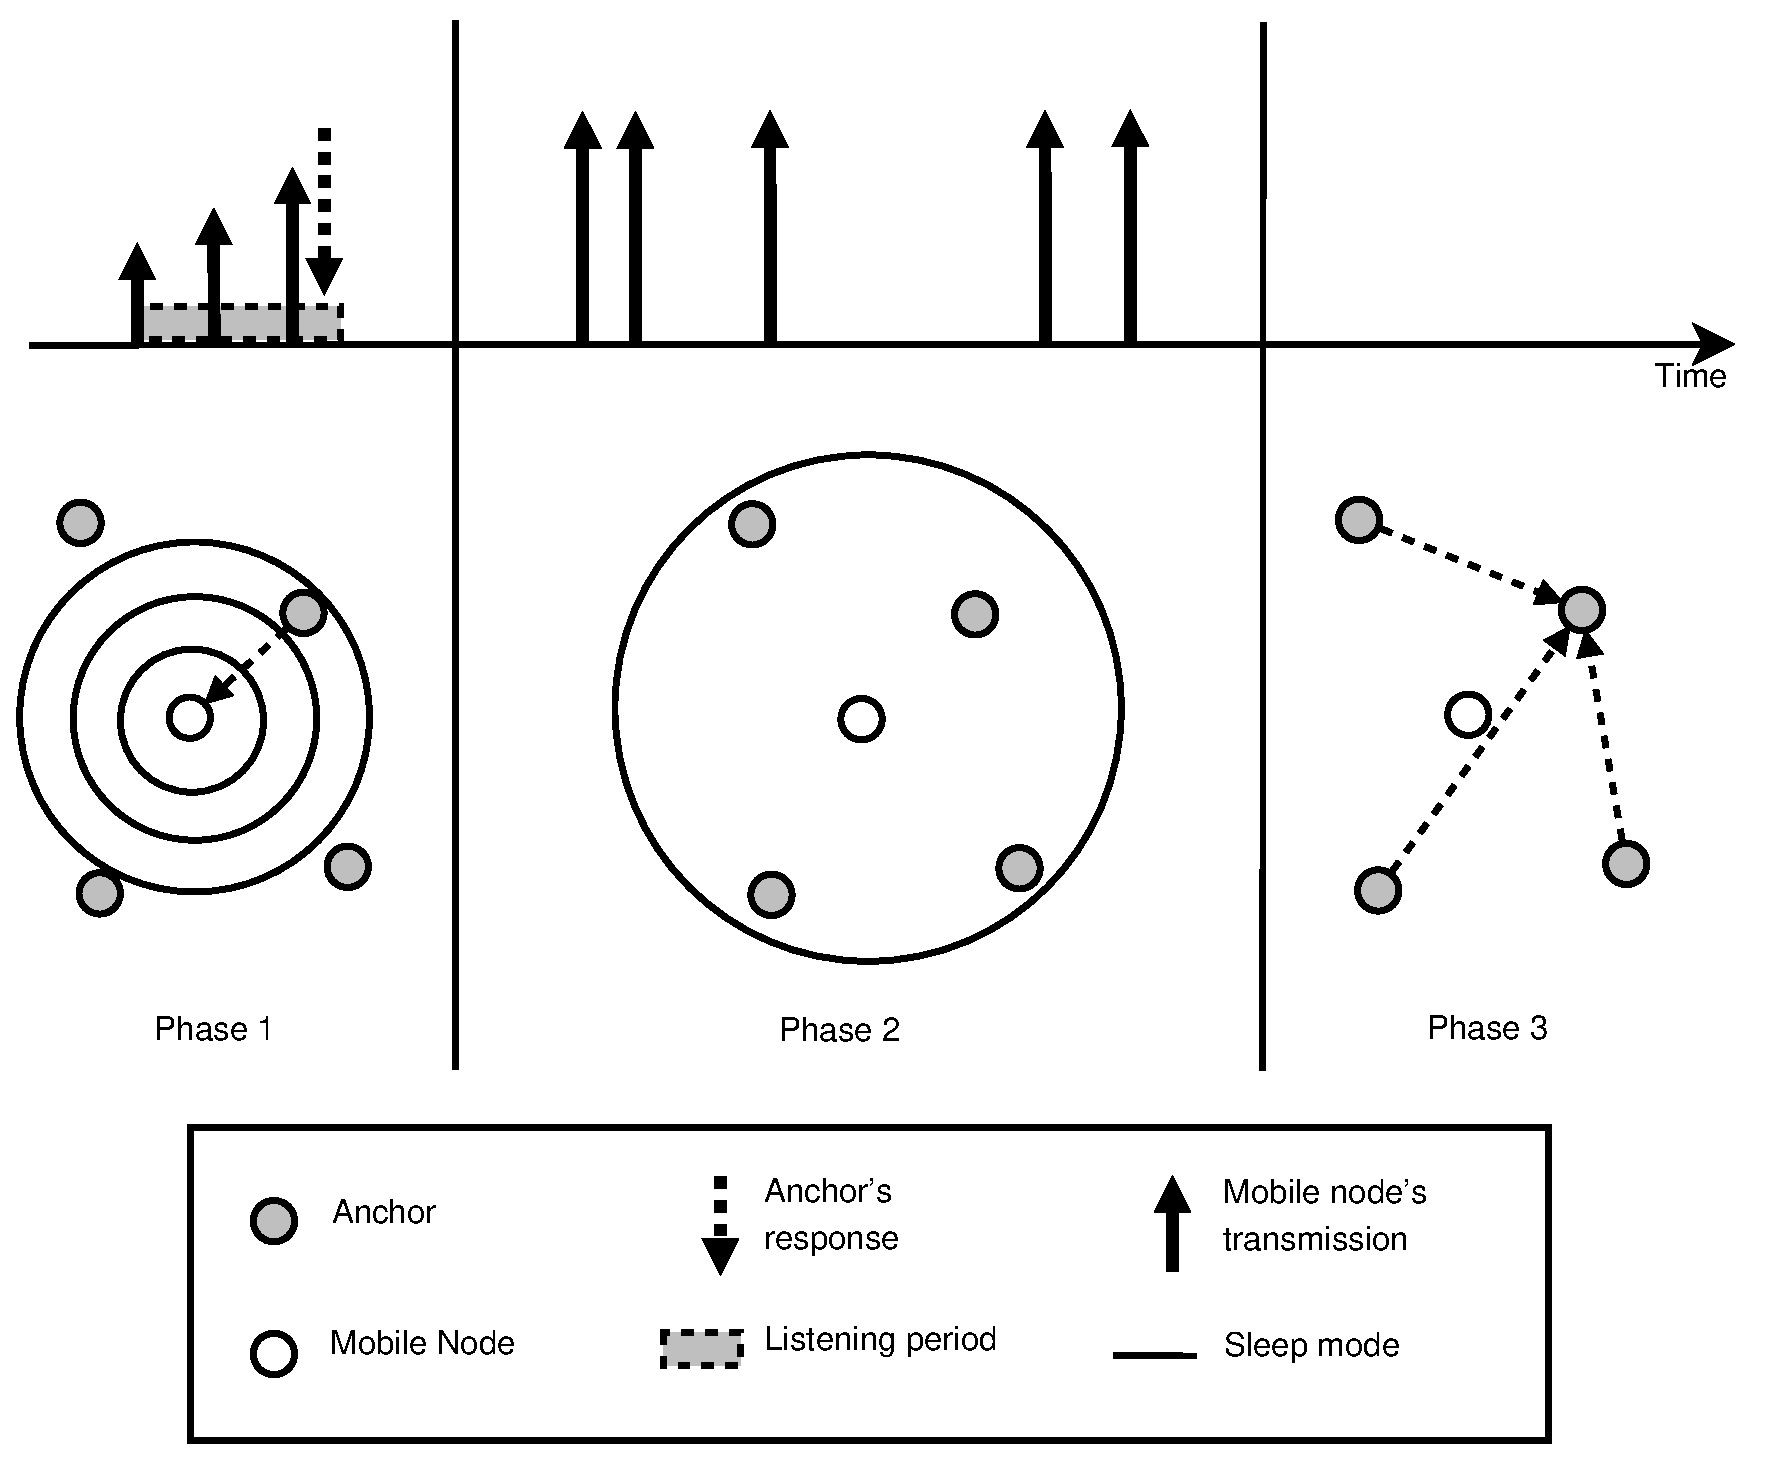
\includegraphics[width=0.7\textwidth]{LPL.eps}
 \end{center}
 \caption{LPL Phases \cite{LPLandOLP}}
 \label{fig:LPL}
\end{figure}

\begin{itemize}
 \item \textbf{Phase 1:} In this phase, \ac{MN} selects a random time to broadcast a synchronization request, starting with the minimum power,
and increasing this power until it receives an answer from an \ac{AN}, this will be the selected \ac{AN}, and the answer will contain information
about the phase times. This process makes sure that only the nearest \acp{AN} answer to this synchronization request. In the next phase 1, if 
the \ac{MN} needs to know its position, it asks its selected \ac{AN} about this information, and if not it just synchronizes.
 \item \textbf{Phase 2:} In phase 2, the \ac{MN} broadcasts several packets in random times to minimize the collisions. Any time the node is not
transmitting, it goes to sleep, this makes that \acp{MN} are awake only when they transmit eliminating this way the idle listening. The \acp{AN} that
received this broadcasts, store the read \ac{RSSI} values and the selected \ac{AN}.
 \item \textbf{Phase 3:} During this phase, the \acp{MN} sleeps and the \acp{AN} send the measured \ac{RSSI} values to the selected \ac{AN}. 
This \ac{AN} will calculate the \ac{MN} position in Distributed-A case or send the data to a central computer in Centralized case. In this phase is
also done the synchronization between \acp{AN} and network configuration.


\end{itemize}


\subsection{\acl{OLP}}

In the case of \ac{OLP} protocol and unlike \ac{LPL}, the \ac{MN} is the one who listens. This protocol is also divided in 3 phases, 2 of 
them can be appreciated in Figure \ref{fig:OLP}.

\begin{figure}[ht]
 \begin{center}
  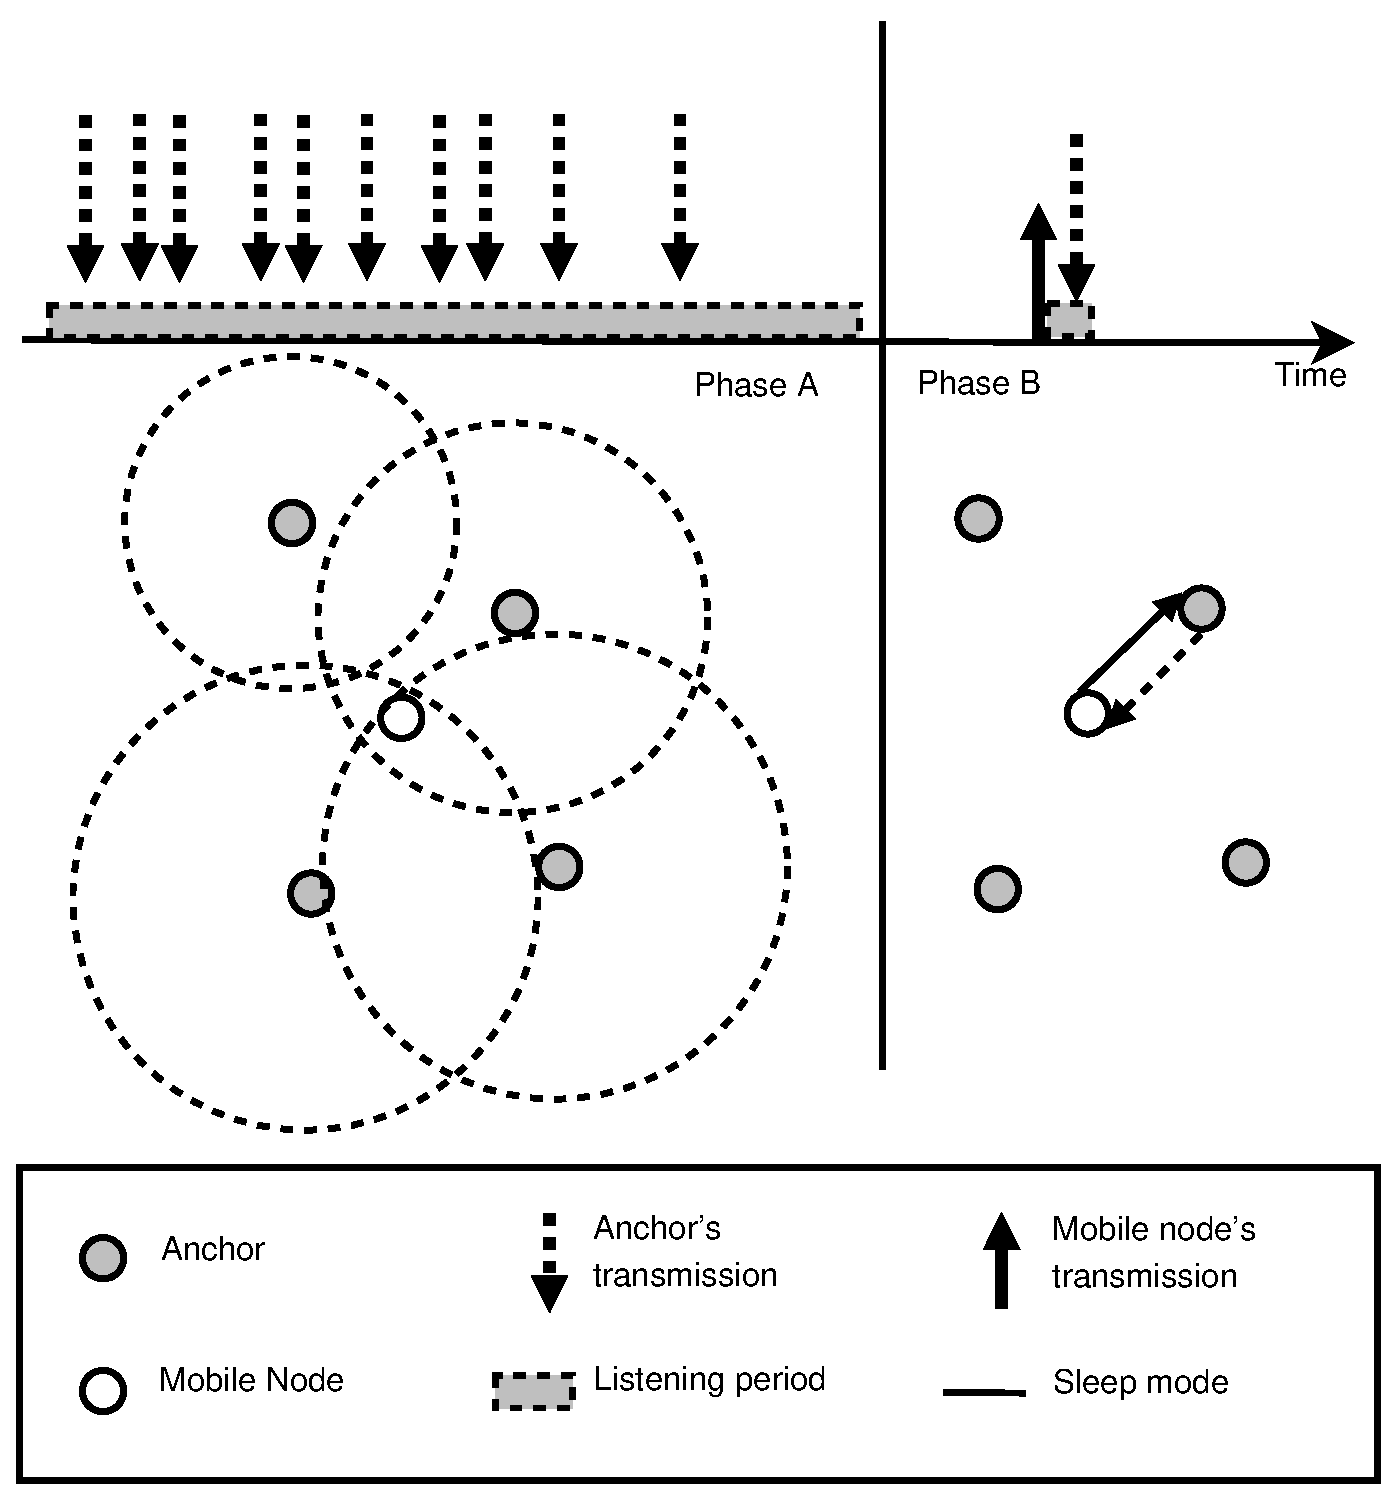
\includegraphics[width=0.5\textwidth]{OLP.eps}
 \end{center}
 \caption{OLP Phases \cite{LPLandOLP}}
 \label{fig:OLP}
\end{figure}

\begin{itemize}
 \item \textbf{Phase A:} In this phase, and thanks to the synchronization among \acp{AN}, the inter-arrival time is reduced, reducing so the
idle listening. This packets also content synchronization information for the \ac{MN}. In this phase \ac{RSSI} values are received and stored
by the \ac{MN}, and then it goes to sleep.
 \item \textbf{Phase B:} In this phase and in Distributed-M mode, the \ac{MN} will use easy localization algorithms together with all the \ac{RSSI}
values read to get its position. In case of Distributed-A or Centralized mode, the \ac{MN} will send a report to the selected \ac{AN}, took 
from the highest \ac{RSSI} value, with all the stored \ac{RSSI} values in Phase A. The selected \ac{AN} will answer with an \ac{ACK}. In next
phase B, the \ac{MN} will ask the selected \ac{AN} about its position in case it needs it.
 \item \textbf{Phase C:} Like in \ac{LPL} this Phase is reserved for communication among \acp{AN} and network configuration.
\end{itemize}


\section{High Configurable Protocol proposal}

From the previous section and according to the results in \cite{LPLandOLP}:
\begin{quote}
``LPL consumes lower energy than OLP when many RSSI samples are required from many ANs. On the other hand,
OLP becomes more energy efficient than LPL when there are several MNs and few RSSI samples are needed. \cite{LPLandOLP}''
\end{quote}

This makes clear the necessity of a Configurable Protocol able to vary the nodes behavior according to the current situation of the network
and the necessities of the node.

High correlation between RSSI values near in time.

Synchronization in the phases.

Centralized vs. Distributed.

Too much time listening to transmit, reduce cases with CSMA when battery is critic using broadcasts from nodes.

As it was seen, \ac{OLP} and \ac{LPL} protocols, are based in \ac{RSSI} values
This work is also based in localization using \ac{RSSI} values, although this work just proposes a framework for the protocol and does not try 
to locate any
node 
From the Table \ref{tab:wsn_applications} (page~\pageref{tab:wsn_applications}) where different applications for \ac{WSN} where stated, it is possible
to extract 4 different kind of nodes.

\section{Sync Phase detail}
